% Created by tikzDevice version 0.10.1 on 2016-06-30 12:57:41
% !TEX encoding = UTF-8 Unicode
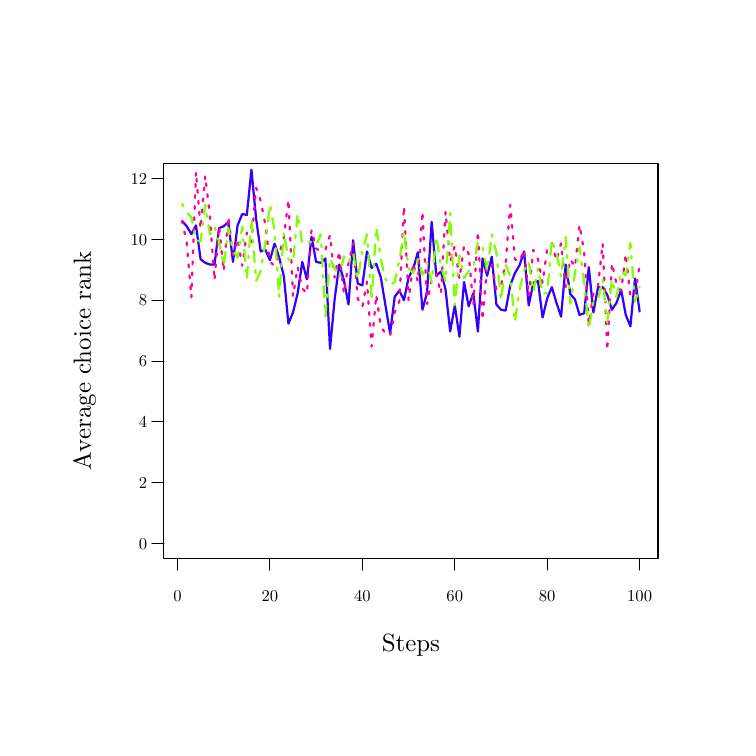
\begin{tikzpicture}[x=1pt,y=1pt]
\definecolor{fillColor}{RGB}{255,255,255}
\path[use as bounding box,fill=fillColor,fill opacity=0.00] (0,0) rectangle (252.94,252.94);
\begin{scope}
\path[clip] ( 49.20, 61.20) rectangle (227.75,203.75);
\definecolor{drawColor}{RGB}{51,0,255}

\path[draw=drawColor,line width= 0.8pt,line join=round,line cap=round] ( 55.81,183.07) --
	( 57.48,181.18) --
	( 59.15,178.35) --
	( 60.82,181.50) --
	( 62.49,169.24) --
	( 64.16,167.98) --
	( 65.83,167.35) --
	( 67.50,167.35) --
	( 69.17,180.55) --
	( 70.84,181.18) --
	( 72.51,182.75) --
	( 74.18,168.30) --
	( 75.85,181.50) --
	( 77.52,185.58) --
	( 79.19,185.27) --
	( 80.86,201.61) --
	( 82.53,184.01) --
	( 84.20,172.07) --
	( 85.87,172.70) --
	( 87.54,168.93) --
	( 89.21,174.90) --
	( 90.88,169.87) --
	( 92.55,163.27) --
	( 94.22,145.99) --
	( 95.89,150.07) --
	( 97.56,156.98) --
	( 99.23,168.30) --
	(100.90,162.01) --
	(102.57,177.41) --
	(104.24,168.30) --
	(105.91,167.98) --
	(107.58,169.55) --
	(109.25,136.87) --
	(110.92,154.78) --
	(112.59,167.35) --
	(114.26,161.70) --
	(115.93,152.90) --
	(117.60,176.15) --
	(119.27,160.44) --
	(120.94,159.81) --
	(122.61,172.07) --
	(124.28,166.10) --
	(125.95,167.67) --
	(127.62,162.64) --
	(129.29,152.58) --
	(130.96,142.53) --
	(132.63,155.73) --
	(134.30,157.93) --
	(135.97,154.47) --
	(137.64,162.64) --
	(139.31,165.78) --
	(140.98,171.75) --
	(142.65,151.01) --
	(144.32,157.30) --
	(145.99,182.75) --
	(147.66,163.27) --
	(149.33,164.84) --
	(151.00,158.24) --
	(152.67,143.16) --
	(154.34,152.58) --
	(156.01,141.27) --
	(157.68,161.07) --
	(159.35,152.27) --
	(161.02,156.98) --
	(162.69,143.16) --
	(164.36,169.55) --
	(166.03,163.27) --
	(167.70,170.18) --
	(169.37,152.90) --
	(171.04,151.01) --
	(172.71,150.70) --
	(174.38,159.81) --
	(176.05,164.21) --
	(177.71,167.04) --
	(179.38,172.07) --
	(181.05,152.58) --
	(182.72,160.76) --
	(184.39,161.38) --
	(186.06,148.19) --
	(187.73,155.10) --
	(189.40,159.18) --
	(191.07,153.53) --
	(192.74,148.50) --
	(194.41,167.35) --
	(196.08,156.67) --
	(197.75,154.78) --
	(199.42,149.13) --
	(201.09,149.76) --
	(202.76,166.41) --
	(204.43,150.07) --
	(206.10,159.18) --
	(207.77,159.18) --
	(209.44,156.36) --
	(211.11,151.01) --
	(212.78,153.53) --
	(214.45,158.24) --
	(216.12,149.13) --
	(217.79,145.04) --
	(219.46,162.33) --
	(221.13,150.38);
\end{scope}
\begin{scope}
\path[clip] (  0.00,  0.00) rectangle (252.94,252.94);
\definecolor{drawColor}{RGB}{0,0,0}

\path[draw=drawColor,line width= 0.4pt,line join=round,line cap=round] ( 54.14, 61.20) -- (221.13, 61.20);

\path[draw=drawColor,line width= 0.4pt,line join=round,line cap=round] ( 54.14, 61.20) -- ( 54.14, 56.92);

\path[draw=drawColor,line width= 0.4pt,line join=round,line cap=round] ( 87.54, 61.20) -- ( 87.54, 56.92);

\path[draw=drawColor,line width= 0.4pt,line join=round,line cap=round] (120.94, 61.20) -- (120.94, 56.92);

\path[draw=drawColor,line width= 0.4pt,line join=round,line cap=round] (154.34, 61.20) -- (154.34, 56.92);

\path[draw=drawColor,line width= 0.4pt,line join=round,line cap=round] (187.73, 61.20) -- (187.73, 56.92);

\path[draw=drawColor,line width= 0.4pt,line join=round,line cap=round] (221.13, 61.20) -- (221.13, 56.92);

\node[text=drawColor,anchor=base,inner sep=0pt, outer sep=0pt, scale=  0.60] at ( 54.14, 45.60) {0};

\node[text=drawColor,anchor=base,inner sep=0pt, outer sep=0pt, scale=  0.60] at ( 87.54, 45.60) {20};

\node[text=drawColor,anchor=base,inner sep=0pt, outer sep=0pt, scale=  0.60] at (120.94, 45.60) {40};

\node[text=drawColor,anchor=base,inner sep=0pt, outer sep=0pt, scale=  0.60] at (154.34, 45.60) {60};

\node[text=drawColor,anchor=base,inner sep=0pt, outer sep=0pt, scale=  0.60] at (187.73, 45.60) {80};

\node[text=drawColor,anchor=base,inner sep=0pt, outer sep=0pt, scale=  0.60] at (221.13, 45.60) {100};

\path[draw=drawColor,line width= 0.4pt,line join=round,line cap=round] ( 49.20, 66.48) -- ( 49.20,198.47);

\path[draw=drawColor,line width= 0.4pt,line join=round,line cap=round] ( 49.20, 66.48) -- ( 44.92, 66.48);

\path[draw=drawColor,line width= 0.4pt,line join=round,line cap=round] ( 49.20, 88.48) -- ( 44.92, 88.48);

\path[draw=drawColor,line width= 0.4pt,line join=round,line cap=round] ( 49.20,110.47) -- ( 44.92,110.47);

\path[draw=drawColor,line width= 0.4pt,line join=round,line cap=round] ( 49.20,132.47) -- ( 44.92,132.47);

\path[draw=drawColor,line width= 0.4pt,line join=round,line cap=round] ( 49.20,154.47) -- ( 44.92,154.47);

\path[draw=drawColor,line width= 0.4pt,line join=round,line cap=round] ( 49.20,176.47) -- ( 44.92,176.47);

\path[draw=drawColor,line width= 0.4pt,line join=round,line cap=round] ( 49.20,198.47) -- ( 44.92,198.47);

\node[text=drawColor,anchor=base east,inner sep=0pt, outer sep=0pt, scale=  0.60] at ( 43.20, 64.41) {0};

\node[text=drawColor,anchor=base east,inner sep=0pt, outer sep=0pt, scale=  0.60] at ( 43.20, 86.41) {2};

\node[text=drawColor,anchor=base east,inner sep=0pt, outer sep=0pt, scale=  0.60] at ( 43.20,108.41) {4};

\node[text=drawColor,anchor=base east,inner sep=0pt, outer sep=0pt, scale=  0.60] at ( 43.20,130.41) {6};

\node[text=drawColor,anchor=base east,inner sep=0pt, outer sep=0pt, scale=  0.60] at ( 43.20,152.40) {8};

\node[text=drawColor,anchor=base east,inner sep=0pt, outer sep=0pt, scale=  0.60] at ( 43.20,174.40) {10};

\node[text=drawColor,anchor=base east,inner sep=0pt, outer sep=0pt, scale=  0.60] at ( 43.20,196.40) {12};

\path[draw=drawColor,line width= 0.4pt,line join=round,line cap=round] ( 49.20, 61.20) --
	(227.75, 61.20) --
	(227.75,203.75) --
	( 49.20,203.75) --
	( 49.20, 61.20);
\end{scope}
\begin{scope}
\path[clip] (  0.00,  0.00) rectangle (252.94,252.94);
\definecolor{drawColor}{RGB}{0,0,0}

\node[text=drawColor,anchor=base,inner sep=0pt, outer sep=0pt, scale=  0.90] at (138.47, 27.60) {Steps};

\node[text=drawColor,rotate= 90.00,anchor=base,inner sep=0pt, outer sep=0pt, scale=  0.90] at ( 22.80,132.47) {Average choice rank};
\end{scope}
\begin{scope}
\path[clip] ( 49.20, 61.20) rectangle (227.75,203.75);
\definecolor{drawColor}{RGB}{255,0,153}

\path[draw=drawColor,line width= 0.8pt,dash pattern=on 1pt off 3pt ,line join=round,line cap=round] ( 55.81,183.16) --
	( 57.48,175.03) --
	( 59.15,155.43) --
	( 60.82,200.86) --
	( 62.49,180.29) --
	( 64.16,199.42) --
	( 65.83,185.08) --
	( 67.50,161.64) --
	( 69.17,181.25) --
	( 70.84,164.99) --
	( 72.51,184.60) --
	( 74.18,170.73) --
	( 75.85,176.47) --
	( 77.52,166.90) --
	( 79.19,178.86) --
	( 80.86,175.51) --
	( 82.53,195.12) --
	( 84.20,190.34) --
	( 85.87,181.73) --
	( 87.54,168.34) --
	( 89.21,166.90) --
	( 90.88,171.21) --
	( 92.55,176.95) --
	( 94.22,190.81) --
	( 95.89,155.90) --
	( 97.56,166.43) --
	( 99.23,158.77) --
	(100.90,156.86) --
	(102.57,179.82) --
	(104.24,173.12) --
	(105.91,172.16) --
	(107.58,172.64) --
	(109.25,177.90) --
	(110.92,162.60) --
	(112.59,172.16) --
	(114.26,156.86) --
	(115.93,167.86) --
	(117.60,175.03) --
	(119.27,154.95) --
	(120.94,152.08) --
	(122.61,161.17) --
	(124.28,137.73) --
	(125.95,156.38) --
	(127.62,144.91) --
	(129.29,142.51) --
	(130.96,141.56) --
	(132.63,150.17) --
	(134.30,153.99) --
	(135.97,188.42) --
	(137.64,154.47) --
	(139.31,167.86) --
	(140.98,161.17) --
	(142.65,186.51) --
	(144.32,153.04) --
	(145.99,162.12) --
	(147.66,164.03) --
	(149.33,156.86) --
	(151.00,186.51) --
	(152.67,168.34) --
	(154.34,174.08) --
	(156.01,162.12) --
	(157.68,174.08) --
	(159.35,171.21) --
	(161.02,152.56) --
	(162.69,179.34) --
	(164.36,147.30) --
	(166.03,166.90) --
	(167.70,167.38) --
	(169.37,158.30) --
	(171.04,159.73) --
	(172.71,167.86) --
	(174.38,188.90) --
	(176.05,169.29) --
	(177.71,168.34) --
	(179.38,172.64) --
	(181.05,155.90) --
	(182.72,172.64) --
	(184.39,169.29) --
	(186.06,160.69) --
	(187.73,173.12) --
	(189.40,175.03) --
	(191.07,168.82) --
	(192.74,175.03) --
	(194.41,159.25) --
	(196.08,169.29) --
	(197.75,166.43) --
	(199.42,181.73) --
	(201.09,171.69) --
	(202.76,145.86) --
	(204.43,156.86) --
	(206.10,159.73) --
	(207.77,175.03) --
	(209.44,136.30) --
	(211.11,167.86) --
	(212.78,160.21) --
	(214.45,157.82) --
	(216.12,171.21) --
	(217.79,155.90) --
	(219.46,156.38) --
	(221.13,167.38);
\definecolor{drawColor}{RGB}{128,255,0}

\path[draw=drawColor,line width= 0.8pt,dash pattern=on 1pt off 3pt on 4pt off 3pt ,line join=round,line cap=round] ( 55.81,189.26) --
	( 57.48,186.19) --
	( 59.15,184.40) --
	( 60.82,176.21) --
	( 62.49,175.70) --
	( 64.16,189.00) --
	( 65.83,178.26) --
	( 67.50,181.07) --
	( 69.17,175.44) --
	( 70.84,167.00) --
	( 72.51,180.56) --
	( 74.18,172.38) --
	( 75.85,169.82) --
	( 77.52,181.07) --
	( 79.19,162.14) --
	( 80.86,183.89) --
	( 82.53,161.38) --
	( 84.20,164.96) --
	( 85.87,175.19) --
	( 87.54,189.00) --
	( 89.21,179.54) --
	( 90.88,155.49) --
	( 92.55,179.03) --
	( 94.22,169.31) --
	( 95.89,168.28) --
	( 97.56,185.68) --
	( 99.23,174.93) --
	(100.90,175.70) --
	(102.57,175.44) --
	(104.24,174.42) --
	(105.91,178.26) --
	(107.58,148.59) --
	(109.25,169.56) --
	(110.92,165.98) --
	(112.59,162.66) --
	(114.26,170.33) --
	(115.93,168.03) --
	(117.60,171.61) --
	(119.27,162.14) --
	(120.94,172.38) --
	(122.61,178.26) --
	(124.28,154.21) --
	(125.95,180.82) --
	(127.62,169.31) --
	(129.29,162.14) --
	(130.96,159.84) --
	(132.63,161.12) --
	(134.30,168.79) --
	(135.97,179.28) --
	(137.64,165.98) --
	(139.31,164.19) --
	(140.98,169.31) --
	(142.65,163.68) --
	(144.32,168.03) --
	(145.99,160.86) --
	(147.66,177.49) --
	(149.33,167.00) --
	(151.00,161.12) --
	(152.67,185.93) --
	(154.34,152.68) --
	(156.01,170.58) --
	(157.68,162.40) --
	(159.35,164.96) --
	(161.02,166.24) --
	(162.69,175.44) --
	(164.36,173.91) --
	(166.03,164.96) --
	(167.70,178.26) --
	(169.37,171.61) --
	(171.04,154.47) --
	(172.71,167.26) --
	(174.38,163.17) --
	(176.05,146.54) --
	(177.71,158.05) --
	(179.38,165.21) --
	(181.05,168.28) --
	(182.72,157.54) --
	(184.39,165.98) --
	(186.06,156.77) --
	(187.73,157.03) --
	(189.40,176.21) --
	(191.07,171.61) --
	(192.74,162.91) --
	(194.41,177.24) --
	(196.08,153.19) --
	(197.75,164.19) --
	(199.42,173.65) --
	(201.09,160.86) --
	(202.76,143.98) --
	(204.43,153.96) --
	(206.10,154.73) --
	(207.77,162.14) --
	(209.44,146.54) --
	(211.11,161.89) --
	(212.78,155.49) --
	(214.45,164.96) --
	(216.12,163.42) --
	(217.79,175.19) --
	(219.46,153.96) --
	(221.13,159.33);
\end{scope}
\end{tikzpicture}
